\subsection{1998 World cup traces}\label{sec:world-cup-1998}

The 1998 World cup traces\cite{ita-wcweb98} are one of the largest
publically available web traces.  They were collected from the many
web servers for the 1998 World Cup games.  We converted the traces
from the special raw format used for them into DataSeries, and also
created a version of the {\tt checklog} program that comes with the
traces as a comparison point for analysis.  For these traces, we found
that conversion to DataSeries files were on average 0.93$\times$ the
size of the original files, and that the analysis program used about
YY$\times$ less CPU time and ran about ZZ$\times$ faster.
% YY = 1.5, ZZ = 2 on my laptop

\subsubsection{Conversion to and from DataSeries}

The conversion to and from DataSeries was quite straightforward.  The
traces use a simple fixed record format of 4 32 bit integers and 4 8
bit integers.  The integers are unsigned in the original format, but
since DataSeries only supports signed 32 bit integers, we converted
to a signed format, and convert backwards during analysis.  

As with most of our converters, we convert both backwards and forwards
to verify that the conversion was correct.  The conversion results
turned out to be very strange; while overall DataSeries compressed 2\%
better, some of the files ended up being smaller while others ended up
being larger.  Further examination identified five factors that were 
affecting the file size:

\begin{itemize}

\item {\bf Compression level}.  The original gzipped World Cup files were
compressed using {\tt gzip -6}, as that is the default compression
level.  DataSeries files default to {\tt gzip -9}.  We simply
re-compressed all of the original files as level 9.  However, this
points out the importance of defaults as people have been downloading
and using needlessly oversized files since they were released.

\item {\bf Endianness}.  The original World Cup files were stored 
in big-endian format.  DataSeries files are stored in the native
endianness of the host, which on x86 processors is little-endian.

\item {\bf Field order}.  The original World Cup files were stored
with the four 32-bit fields first and then the 4 8-bit fields.
DataSeries happened to store the files with all the 8-bit fields first
followed by the 32-bit ones.

\item {\bf Field padding}.  The original World Cup files included
no padding.  DataSeries padded the files to an 8 byte boundary, so
added in an extra 4 bytes of zeros to each record.

\item {\bf Relative field packing}.  The original World Cup files stored
the time field as absolute seconds.  DataSeries includes an option to
store fields calculated relative to the previous value.

\end{itemize}

Table~\ref{table:wc1998:compression} shows the overall compression of
the different options.  The \{le,be\}-\{bts,stb\}-gz files are the
original data files stored in little or big endian format (le/be) and
big to small or small to big (bts/stb) ordering.  The original traces
are be-bts-gz.  The DataSeries file without any options is ds-base,
and then options can be added on for reducing the field padding to the
maximum column size (mcs), packing the fields in big to small order
(bts), or packing the time field self-relative (tsr).

% plots and tables can be re-generated using graphs/wc1998/plot.hg
% files can be re-generated by running wcweb2ds with an extent size of 1000000
% and by changing pack_ to xack_ in the type definition.

\begin{table}
\centering
\begin{tabular}{|c|c|c|c|}\hline

               &            & ratio to & ratio to  \\
    dataset    & size (MiB) & ds-base  & be-bts-gz \\
\hline							   
ds-mcs-bts-tsr & 7648.98    & 1.133    & 1.077     \\
ds-mcs-tsr     & 7722.78    & 1.122    & 1.067     \\
ds-bts-tsr     & 7890.12    & 1.098    & 1.044     \\
ds-tsr         & 8065.99    & 1.074    & 1.021     \\
le-bts-gz      & 8152.47    & 1.063    & 1.011     \\
ds-mcs-bts     & 8183.98    & 1.059    & 1.007     \\
be-bts-gz      & 8239.15    & 1.052    & 1.000     \\
le-stb-gz      & 8391.09    & 1.032    & 0.982     \\
be-stb-gz      & 8411.46    & 1.030    & 0.980     \\
ds-mcs         & 8423.56    & 1.029    & 0.978     \\
ds-bts         & 8439.72    & 1.027    & 0.976     \\
ds-base        & 8663.78    & 1.000    & 0.951     \\
\hline
\end{tabular}


\caption{Compression options for the data files sorted from the smallest 
to the largest.  Gzipped files can be stored little or big endian
(le/be) and small to big or big to small (stb/bts).  DataSeries files
can be stored with the fields padded only to the maximum column size
(mcs), with the fields stored big to small (bts), or with the time
field packed self relative (tsr). be-bts-gz is the original 1998 World
Cup trace format.}

\label{table:wc1998:compression}
\end{table}

\subsubsection{Original file compression experiments}

\begin{figure}
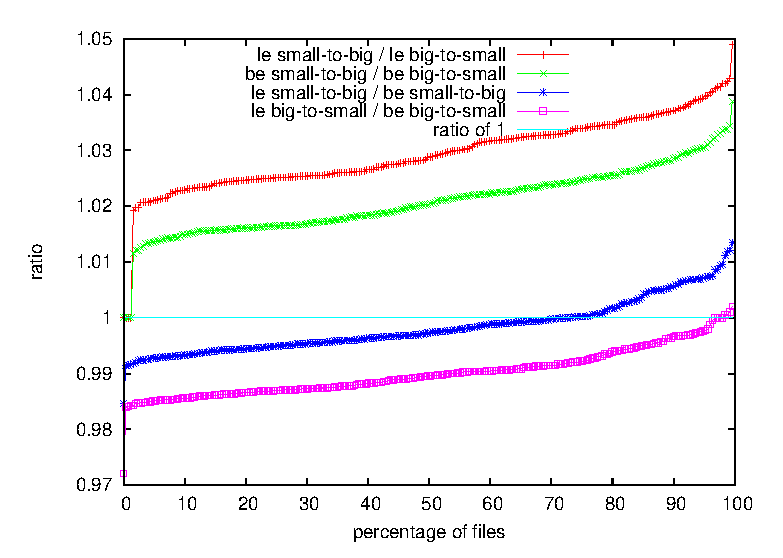
\epsfig{width=3.2in, angle=0, file=graphs/wc1998/reordering-options.ps}
\caption{Reordering options for the original data files.  
The data can be stored in little or big endian format (le/be); it can
also be stored with the small fields before the big ones or the
reverse (stb/bts)}
\label{fig:wc1998:original-data-reordering}
\end{figure}

Figure~\ref{fig:wc1998:original-data-reordering} shows the four
possible options for packing the data before compression in the
original data format.  Since the dataset includes some empty fields,
we always get some files that compress the same regardless of the
packing (to 20 bytes, the minimal gzip file size). 

The top two lines compare the small to big and big to small ordering
options holding the endianness constant.  Since both lines are
entirely positive, this shows us that we always prefer the
big-to-small ordering for this dataset (if the ratio is $>$ 1 then the
denominator is smaller and hence the preferrable choice), regardless
of endianness.  However, we note that changing the ordering makes more
of a difference if the files are little endian.

The bottom two lines compare the endianness choices holding the field
ordering constant.  Since the lines are mostly below zero, we in
gneneral prefer the little endian files to the big endian files, and
the preference is more pronounced for the big-to-small ordering.

\subsubsection{DataSeries file compression experiments}

The first DataSeries graph looks at the overhead imposed by the
DataSeries file format.  For this experiment, we pruned out the 5 tiny
files (4 empty, and 1 $<$4k compressed) in the dataset as DataSeries
imposes a large overhead on very tiny files since it includes the type
information in each file.  In particular, for an empty file, the
overhead is about 80x as at DataSeries files are 1.6k and the original
files are 20 bytes.  Figure~\ref{fig:wc1998:ds-overhead} shows
the overhead imposed by DataSeries with both the big-to-small and the
small-to-big orderings for the files, and using $10^6$ byte extent
sizes.  We can see that DataSeries imposes a 0.2\%-0.5\% overhead on
the files if the underlying data is identical.  We manually verified
that a few files were in identical except for the type extent at the
beginning of the file, the extent headers that occurred at the middle
of the files, and the trailer at the end.

\begin{figure}
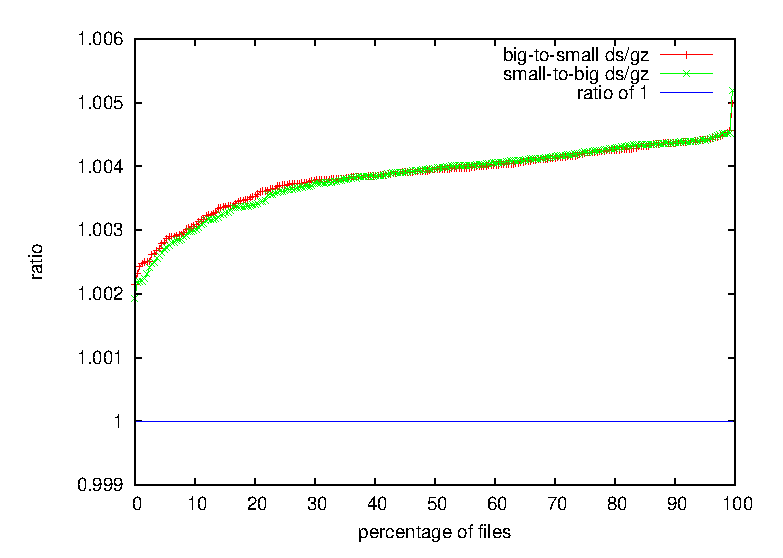
\epsfig{width=3.2in, angle=0, file=graphs/wc1998/ds-overhead.ps}
\caption{Overhead imposed by DataSeries. The record format is constrained
to be identical to the original data.  DataSeries imposes a
0.2\%-0.5\% overhead.}
\label{fig:wc1998:ds-overhead}
\end{figure}

The second graph shown in figure~\ref{fig:wc1998:ds-opts-1} looks
at the effect of the field packing (mcs) and field ordering (bts)
options for DataSeries.  We compare the file sizes measured by turning
on each of the options individually, and then both at the same time.
The results are much as would be expected; eliminating the extra
padding (mcs) gives us a flat 2-3\% compression improvement.
Switching to big-to-small (bts) field ordering gives a 1-4\%.  The
options combine to give us a 5-7\% compression improvement over the
base DataSeries case.  The one oddness is the couple of points that
are below 1.  These come from the empty files.  We changed the options
to the packing by changing the XML option from pack\_* to xack\_* so
as to minimize the change in the size of the type extent.  However,
having all three options specified as xack\_* compresses slightly
better (4 bytes) than having one or two options as pack\_* and the
others as xack\_*, resulting in the negligably below 1 ratio.

\begin{figure}
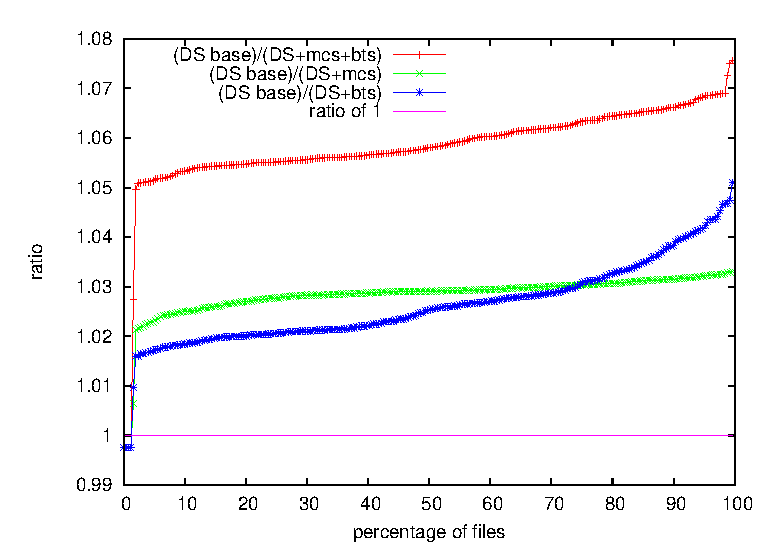
\epsfig{width=3.2in, angle=0, file=graphs/wc1998/ds-opts-1.ps}
\caption{Turning on the field compaction (mcs) and ordering (bts) options 
in DataSeries.  The compression options are mostly independent, so the
resulting compression of turning both on is multiplicative.}
\label{fig:wc1998:ds-opts-1}
\end{figure}

The third graph shown in figure~\ref{fig:wc1998:ds-opts-2} looks
at the effect of the time self-relative packing option and then
combines it with the field packing (mcs) and field ordering (bts)
options.  Time self relative gives a much more substantial improvement
in some cases -- by itself it can give a 20\% compression improvement.
However it does not operate nearly as independently as the first two
options, in particular turning on both bts and mcs packing is not much
of an improvement over just mcs packing.

\begin{figure}
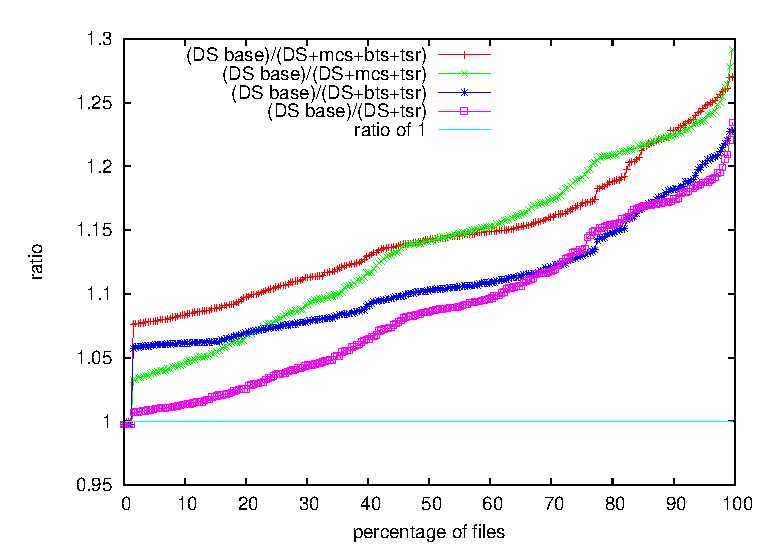
\epsfig{width=3.2in, angle=0, file=graphs/wc1998/ds-opts-2.ps}
\caption{Turning on the time self-relative (tsr) option and then the 
field compaction (mcs) and ordering (bts) options in DataSeries.  
With time self-relative packing, the options are no longer independent, 
and overall time self-relative gives a much more substantial improvement 
than the other options.}
\label{fig:wc1998:ds-opts-2}
\end{figure}

The fourth graph shown in figure~\ref{fig:wc1998:ds-opts-3} looks at
just the effect of turning on the big-to-small packing option with the
field compaction (mcs) and time self-relative (tsr) options already
turned on.  This graph shows why the benefit of big-to-small is so
minor once the other options are on.  The big-to-small option
interferes in some cases with the time self-relative option.  This
figure leads to the idea that different extents could be packed using
different field orderings as in DataSeries, each extent boundary could
be stored in different ways.

\begin{figure}
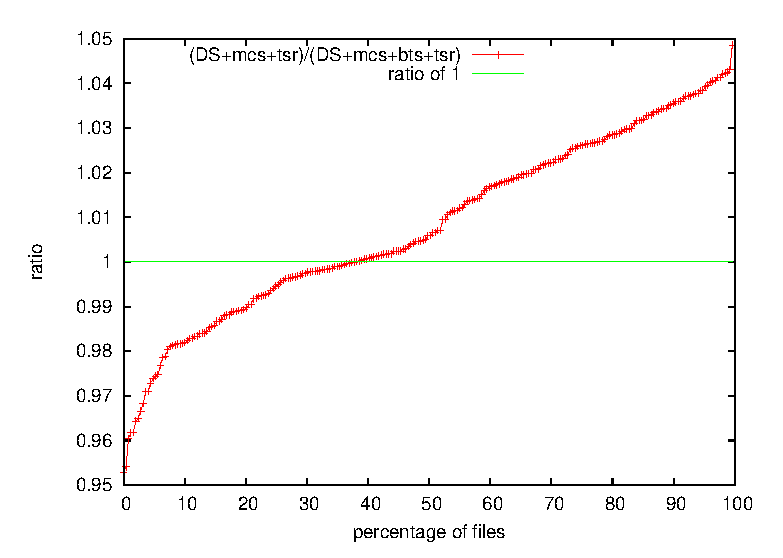
\epsfig{width=3.2in, angle=0, file=graphs/wc1998/ds-opts-3.ps}
\caption{Comparing just the field ordering option (bts) with both the
time self-relative (tsr) and field compaction (mcs) options enabled.
Packing big to small is a win, but not by much.}
\label{fig:wc1998:ds-opts-3}
\end{figure}

The fifth graph shown in figure~\ref{fig:wc1998:ds-size-cmp} looks at
whether or not there is any size correlation to the improvment
provided by the compression options.  Visually the graph shows no
significant correlation between size and compression ratio as the
values are just scattered within a range.

\begin{figure}
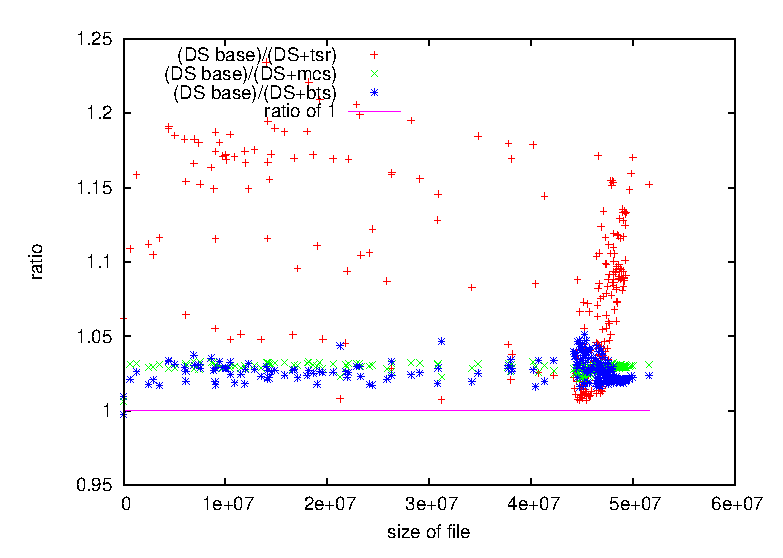
\epsfig{width=3.2in, angle=0, file=graphs/wc1998/ds-size-cmp.ps}
\caption{Determining if any of the compression options correlate with
size of the file.  Visually they do not appear to.}
\label{fig:wc1998:ds-size-cmp}
\end{figure}

\subsubsection{Compression conclusions}

The work in this section showed that the field compaction option had a
small but consistent effect on the compressibility of the data.  We
would recommend that any extent type that does not have any 8 byte
fields always turn on this option.  In fact, the option could be
turned on in general, but it will have no effect (other than consuming
a small amount of space in the extent type) if there are 8 byte fields
in the record type, or if the record size is otherwise a multiple of
8.

The work in this section also shows that field ordering can have a
substantial effect on the compressibility of an extent.  On every
extent boundary, the fields that access the extent get a chance to
re-calculate their offsets into the data.  This means that for graphs
like figure~\ref{fig:wc1998:ds-opts-3} we could in theory make it so
that all files are compressed as well as just having the mcs+tsr
options enabled.  Indeed, just choosing a per-file field ordering that
would match the best ordering for the file would improve the
compression.  However, we could potentially do even better as each
extent in a single file could choose the best ordering.  Moreover, we
have only tested a subset of the possible ordering options.  For this
dataset, there are actually $5!*4!$ possible orderings that don't
introduce additional padding.  This comes from there are 5 32-bit
units (4 actual and 4 8-bit) that could have any order, and then the 4
8-bit values could be ordered in any order.  We hypothesize that
correlations between fields will correlate with the amount of
compression that could be achieved, and hence it may be possible to
work out much better field orderings without evaluating an exponential
number of values.

\subsubsection{Analysis performance}

We re-implemented the {\tt checklog} program that comes with the 1998
World Cup traces.  That program calculates a couple of the values in
multiple ways.  We duplicated this calculation because we wanted the
programs to be comparable, even though performing the calculation is
unnecesary. When running the program we found that the DataSeries
implementation ran ZZ$\times$ faster.  This result was expected as the
analysis performed was fairly simple, and as DataSeries used multiple
CPUs for decompression, it was able to run faster.  However, we also
found that the implementation used about YY$\times$ less CPU.  This
was unexpected given that DataSeries was using a virtual function call
for every row, and was having to process the extents separately.  We
examined the CPU utilization using oprofile and valgrind and found
that the original code had three problems:

\begin{itemize}

\item {\bf Non-integrated decompression}.  The {\tt checklog} program 
used a separate process to perform the decompression, this led to
slightly increased system time to pass the data over the pipe.

\item {\bf Very slow byte-swapping routine}.  The {\tt checklog} program
had to byte-swap every record, and the implementation used for
byte-swapping was very slow.  Moreover, the implementation copied the
data rather than doing the byte-swapping in-place, further increasing
the overhead.

\item {\bf Slow per-record fread}.  The {\tt checklog} program called 
fread for each record.  While we didn't expect this to be slow, it
turned out that the implementation is slow, and so calling fread for
each record is a poor choice.

\end{itemize}

While we could re-implement {\tt checklog}, it doesn't seem
particularly valuable.  The expected end result would be that the
checklog program would use less CPU time than the DataSeries program,
but would use more wall-clock time because there is no easy way to
parallelize the reading of the underlying files.

